%!TEX program = xelatex

\documentclass[11pt]{article}
\usepackage{geometry}
\usepackage{tcolorbox}
\usepackage{hyperref}
\usepackage{microtype}
\usepackage{rotating}
\usepackage[backend=biber,sorting=none,style=apa]{biblatex}
\addbibresource{library.bib}
\geometry{
    a4paper,
    total={170mm,257mm},
    left=20mm,
    top=20mm,
}
\setlength{\parskip}{5pt}
\setlength\parindent{0pt}
\usepackage{graphicx}
\usepackage{booktabs}
\usepackage{subcaption}
\usepackage{amsmath}
\usepackage{amsfonts}
\usepackage{amssymb}
\usepackage{lscape}
\usepackage{psfrag}
\usepackage{hyperref}
\hypersetup{
  colorlinks = false,
  urlcolor   = blue,
  linkcolor  = blue,
  citecolor  = red
}
\usepackage{verbatim}
\usepackage{textcomp}
\usepackage{multirow}
\usepackage{rotating}
\usepackage{adjustbox}
\usepackage{tikz}
\usepackage[english]{babel}
\usepackage{appendix}
\usepackage{parskip}
\usepackage{placeins}
\usepackage[tableposition=top]{caption}
\captionsetup{skip=0pt}

\usepackage{amsmath}
\usepackage{fontspec}
\usepackage[charter]{newtxmath}

\setmainfont{XCharter}
\newfontfamily{\XCharterLF}{XCharter}[NFSSFamily=xcharterlf]

\DeclareSymbolFont{operators}{TU}{xcharterlf}{m}{n}

\usepackage{listings}
\lstset{
  language=R,
  basicstyle=\footnotesize,
  numbers=left,
  numberstyle=\tiny,
  numbersep=5pt,
  showstringspaces=false,
  frame=single
} 

\sloppy
\widowpenalty=10000
\clubpenalty=10000
\edef\today{%\number\day\
\ifcase\month\or
January\or February\or March\or April\or May\or June\or July\or
August\or September\or October\or November\or December\fi\ \number\year}
\title{\vspace*{40.0mm}
  \bf\sf Assignment
         \vspace*{20.0mm} \\
  \vspace*{40.0mm}}
\author{\sf Van den Broeck Sebastiaan (r0902562)}
\date{\sf 13/03/2023}

\begin{document}

\begin{figure}
  \parbox[t]{125mm}{
    \vspace*{6mm}
    \scriptsize\sf           FACULTY OF SCIENCE \\
    \scriptsize\sf           DEPARTMENT OF MATHEMATICS \\
    \scriptsize\sf\bfseries  MASTER OF STATISTICS AND DATA SCIENCE \\
    \scriptsize\sf\bfseries  STRUCTURAL EQUATION MODELING \\}
  \parbox[t]{40mm}{
    \begin{flushright}
      
\includegraphics[height=15mm]{logo.eps.pdf}
    \end{flushright}}
\end{figure}

\maketitle
\thispagestyle{empty}
\raggedbottom

\cleardoublepage
\setcounter{page}{1}
\setcounter{tocdepth}{3}

\section{Introduction}

It has been noted that almost one in six individuals in the United States will
experience a depressive disorder. Consequently, considerable personal, social and
economic loss can be attributed to this type of illness. Although there is clearly
a very large societal impact of depression, little is known about its relationship
with personality and social functioning. In this work I will test a hypothesis
related to depression that has been proposed by \textcite{tse2011}. Specifically,
they proposed that harm avoidance and self-directedness are indirectly linked to
depression through social functioning. Moreover, there should also be a direct effect
of self-directedness on depression. On the one hand, a behaviour can be classified
under harm avoidance if it is done to avoid novelty and punishment. Self-directedness,
on the other hand, is a form of self-determination and ability to regulate behaviour
to suit goals and values. The authors have tested this hypothesis on a sample of
university students, which limits the interpretability of their findings. By
testing their hypothesis on a larger and more representative sample, I hope to
contribute to the literature on depression. The dataset will be discussed next.
Afterwards, a structural equation model has been used to test the hypothesis and
will be discussed as well. Lastly, the results and implications thereof will be
considered.

\section{Preliminaries}
\subsection{Data}

The data treated in this report is the Midlife in the United States (MIDUS)
series. It is a national longitudinal study of health and well-being, created by
a team of multi-disciplinary researchers. Currently, there are three waves in
the study, which were collected via phone interviews, surveys and by bringing
participants into clinical settings to facilitate collecting biological data.
All three waves cover the contiguous United States in its entirety. The first wave
was collected in 1995 and 1996, while the second wave was collected in 2004 and
2005. The most recent and third wave was collected in 2013 and 2014. In this
analysis, the second and third wave have been combined to create a bigger dataset.
It was not possible to incorporate the first wave, since a lot of variables
changed between the first and second and third waves (\cite{radler2014}). In this
section I will discuss the variables that have been used in the analysis.

An important reason for choosing this dataset is that it contains a lot of
documentation for which variables form certain latent constructs such as
depression or social anxiety. Since I am not too familiar with the field of
psychology this would allow me to test a hypothesis that is better grounded in
theory. First, depression is the most important latent variable in this work. It
has been measured through seven questions during which the respondent reflects
over the last two weeks. For example, the questions include losing interest,
becoming tired, having trouble falling asleep or thinking about death. The
responses have been recoded such that a higher score equates a higher level of
depression. Specifically, each variable which measures this latent construct has
been coded such that a 1 reflects a yes answer. As could be expected, a 0 then
means a respondent has answered no.

\begin{table}[h!]
\captionsetup{singlelinecheck=off}
\caption{Depression indicators}
\scalebox{0.8}{
\begin{tabular}{|l|l|l|}
\hline
\textbf{Construct}          & \textbf{Code} & \textbf{Question}                                                                                                                                              \\ \hline
\multirow{7}{*}{Depression} & PA63        & During those two weeks, did you lose interest in most things?                                                                                                  \\ \cline{2-3} 
                            & PA64        & \begin{tabular}[c]{@{}l@{}}Thinking about these same two weeks, did you feel more tired\\ out or low on energy?\end{tabular}                                   \\ \cline{2-3} 
                            & PA65        & During those same two weeks, did you lose appetite?                                                                                                            \\ \cline{2-3} 
                            & PA66        & \begin{tabular}[c]{@{}l@{}}Did you have more trouble falling asleep than you usually do\\ during those two weeks?\end{tabular}                                 \\ \cline{2-3} 
                            & PA67        & \begin{tabular}[c]{@{}l@{}}During that same two week period, did you have a lot more\\ trouble concentrating than usual?\end{tabular}                          \\ \cline{2-3} 
                            & PA68        & \begin{tabular}[c]{@{}l@{}}People sometimes feel down on themselves, no good, or worthless.\\ During that two-week period, did you feel this way?\end{tabular} \\ \cline{2-3} 
                            & PA69        & \begin{tabular}[c]{@{}l@{}}Did you think a lot about death - either your own, someone else's\\ or death in general - during those two weeks?\end{tabular}      \\ \hline
\end{tabular}
}
\end{table}

\begin{table}[h!]
\captionsetup{singlelinecheck=off}
\caption{Depression indicators distribution}
\scalebox{0.8}{
\begin{tabular}{|l|l|ll|}
\hline
\multirow{2}{*}{\textbf{Construct}} & \multirow{2}{*}{\textbf{Code}} & \multicolumn{2}{l|}{\textbf{Count}} \\ \cline{3-4} 
                                    &                                & \multicolumn{1}{l|}{0}      & 1     \\ \hline
\multirow{7}{*}{Depression}         & PA63                         & \multicolumn{1}{l|}{126}    & 479   \\ \cline{2-4} 
                                    & PA64                         & \multicolumn{1}{l|}{51}     & 554   \\ \cline{2-4} 
                                    & PA65                         & \multicolumn{1}{l|}{263}    & 342   \\ \cline{2-4} 
                                    & PA66                         & \multicolumn{1}{l|}{172}    & 433   \\ \cline{2-4} 
                                    & PA67                         & \multicolumn{1}{l|}{88}     & 517   \\ \cline{2-4} 
                                    & PA68                         & \multicolumn{1}{l|}{222}    & 383   \\ \cline{2-4} 
                                    & PA69                         & \multicolumn{1}{l|}{229}    & 376   \\ \hline
\end{tabular}
}
\end{table}

Second, another important aspect in this report is harm avoidance. It has been
described as an inheritable tendency for inhibiting behaviours to avoid novelty
and punishment (\cite{tse2011}). Since it cannot be measured directly, four
questions were asked to get an idea about this construct. First, interviewees
were asked whether they would enjoy experiencing an earthquake or learning to
walk the tightrope. These two variables were reverse recoded such that a 4
reflects not agreeing with the statement at all (harm avoidance), while a 1
indicates fully agreeing (no avoidance). Second, interviewees were presented with
two scenario's twice. For each question, one scenario corresponds to a harmful
situation, while the other scenario's is harmless. Again, there was a recoding
such that a higher score on these two variables indicates avoiding harm.

\begin{table}[h!]
\captionsetup{singlelinecheck=off}
\caption{Harm avoidance indicators}
\scalebox{0.8}{
\begin{tabular}{|l|l|l|}
\hline
\textbf{Construct}              & \textbf{Code} & \textbf{Question}                                                                                                                                                                                                                                                                                                              \\ \hline
\multirow{4}{*}{Harm avoidance} & SE7D        & It might be fun and exciting to be in an earthquake.                                                                                                                                                                                                                                                                           \\ \cline{2-3} 
                                & SE7V        & It might be fun learning to walk a tightrope.                                                                                                                                                                                                                                                                                  \\ \cline{2-3} 
                                & SE8         & \begin{tabular}[c]{@{}l@{}}Of these two situations, I would dislike more: Situation 1: \\ Riding a long stretch of rapids in a canoe; Situation 2:\\ Waiting for someone who's late.\end{tabular}                                                                                                                              \\ \cline{2-3} 
                                & SE9         & \begin{tabular}[c]{@{}l@{}}Of these two situations, I would dislike more: Situation 1:\\ Being at the circus when two lions suddenly get loose\\ down in the ring; Situation 2: Bringing my whole family\\ to the circus and then not being able to get in because a\\ clerk sold me tickets for the wrong night.\end{tabular} \\ \hline
\end{tabular}
}
\end{table}

\begin{table}[h!]
\captionsetup{singlelinecheck=off}
\caption{Harm avoidance distribution}
\scalebox{0.8}{
\begin{tabular}{|l|l|llll|}
\hline
\multirow{2}{*}{\textbf{Construct}} & \multirow{2}{*}{\textbf{Code}} & \multicolumn{4}{l|}{\textbf{Count}}                                                                              \\ \cline{3-6} 
                                    &                                & \multicolumn{1}{l|}{\textbf{1 (harm)}} & \multicolumn{1}{l|}{\textbf{2}} & \multicolumn{1}{l|}{\textbf{3}} & \textbf{4 (no harm)} \\ \hline
\multirow{2}{*}{Harm avoidance}     & SE7D                         & \multicolumn{1}{l|}{33}                  & \multicolumn{1}{l|}{92}         & \multicolumn{1}{l|}{91}         & 389                 \\ \cline{2-6} 
                                    & SE7V                         & \multicolumn{1}{l|}{25}                  & \multicolumn{1}{l|}{79}         & \multicolumn{1}{l|}{69}         & 432                 \\ \hline
\end{tabular}
}
\end{table}

\begin{table}[h!]
\captionsetup{singlelinecheck=off}
\caption{Harm avoidance distribution}
\scalebox{0.8}{
\begin{tabular}{|l|l|ll|}
\hline
\multirow{2}{*}{\textbf{Construct}} & \multirow{2}{*}{\textbf{Code}} & \multicolumn{2}{l|}{\textbf{Count}}          \\ \cline{3-4} 
                                    &                                & \multicolumn{1}{l|}{\textbf{0 (harm)}} & \textbf{1 (no harm)} \\ \hline
\multirow{2}{*}{Harm avoidance}     & SE8                            & \multicolumn{1}{l|}{335}                  & 270       \\ \cline{2-4} 
                                    & SE7V                           & \multicolumn{1}{l|}{276}                  & 329       \\ \hline
\end{tabular}
}
\end{table}

Third, we should not forget about self-directedness, which has been measured
through three variables. It evaluates the amount of self-determination and ability
a respondent has in order to regulate behaviour to achieve goals and values
(\cite{tse2011}). Making plans for the future, knowing what to want out of life
and setting goals are important for this dimension. Again, the variables were
reverse coded such that a higher score reflects agreeing more with the statement.
The data indicates that most participants agree somewhat or fully what the three
statements.

\begin{table}[h!]
\captionsetup{singlelinecheck=off}
\caption{Self-directedness indicators}
\scalebox{0.8}{
\begin{tabular}{|l|l|l|}
\hline
\textbf{Construct}                 & \textbf{Code} & \textbf{Question}                                   \\ \hline
\multirow{3}{*}{Self-directedness} & SE14O       & I like to make plans for the future.                \\ \cline{2-3} 
                                   & SE14R       & I know what I want out of life.                     \\ \cline{2-3} 
                                   & SE14P       & I find it helpful to set goals for the near future. \\ \hline
\end{tabular}
}
\end{table}

\begin{table}[h!]
\captionsetup{singlelinecheck=off}
\caption{Self-directedness distribution}
\scalebox{0.8}{
\begin{tabular}{|l|l|llll|}
\hline
\multirow{2}{*}{\textbf{Construct}} & \multirow{2}{*}{\textbf{Code}} & \multicolumn{4}{l|}{\textbf{Count}}                                                                              \\ \cline{3-6} 
                                    &                                & \multicolumn{1}{l|}{\textbf{1}} & \multicolumn{1}{l|}{\textbf{2}} & \multicolumn{1}{l|}{\textbf{3}} & \textbf{4} \\ \hline
\multirow{3}{*}{Self-directedness}  & SE14O                        & \multicolumn{1}{l|}{48}        & \multicolumn{1}{l|}{140}       & \multicolumn{1}{l|}{241}       & 176       \\ \cline{2-6} 
                                    & SE14R                        & \multicolumn{1}{l|}{67}        & \multicolumn{1}{l|}{144}       & \multicolumn{1}{l|}{235}       & 159       \\ \cline{2-6} 
                                    & SE14P                        & \multicolumn{1}{l|}{47}        & \multicolumn{1}{l|}{149}       & \multicolumn{1}{l|}{228}       & 181       \\ \hline
\end{tabular}
}
\end{table}

Fourth, the latent variable social functioning has been used in the analysis.
Seven questions related to this dimension were asked. The variables SE1BB, SE1D,
SE1I and SE1V were reverse coded such that a higher score indicates a higher
degree of social functioning.  The dataset counts 601 observations after deleting
rows with missing values. A missingness at random principle is therefore assumed.

\begin{table}[h!]
\captionsetup{singlelinecheck=off}
\caption{Social functioning indicators}
\scalebox{0.8}{
\begin{tabular}{|l|l|l|}
\hline
\textbf{Construct}                  & \textbf{Code} & \textbf{Question}                                                                                                                                    \\ \hline
\multirow{7}{*}{Social functioning} & SE1BB       & \begin{tabular}[c]{@{}l@{}}People would describe me as a giving person, willing to share my time \\ with others.\end{tabular}                        \\ \cline{2-3} 
                                    & SE1D        & Most people see me as loving and affectionate.                                                                                                       \\ \cline{2-3} 
                                    & SE1HH       & I have not experienced many warm and trusting relationships with others.                                                                             \\ \cline{2-3} 
                                    & SE1J        & Maintaining close relationships has been difficult and frustrating for me.                                                                           \\ \cline{2-3} 
                                    & SE1P        & \begin{tabular}[c]{@{}l@{}}I often feel lonely because I have few close friends with whom to share my\\ concerns.\end{tabular}                       \\ \cline{2-3} 
                                    & SE1V        & I enjoy personal and mutual conversations with family members and friends.                                                                           \\ \hline
\end{tabular}
}
\end{table}

\begin{table}[h!]
\captionsetup{singlelinecheck=off}
\caption{Social functioning distribution}
\scalebox{0.8}{
\begin{tabular}{|l|l|lllllll|}
\hline
\multirow{2}{*}{\textbf{Construct}} & \multirow{2}{*}{\textbf{Code}} & \multicolumn{7}{l|}{\textbf{Count}}                                                                                                                                                                                    \\ \cline{3-9} 
                                    &                                & \multicolumn{1}{l|}{\textbf{1}} & \multicolumn{1}{l|}{\textbf{2}} & \multicolumn{1}{l|}{\textbf{3}} & \multicolumn{1}{l|}{\textbf{4}} & \multicolumn{1}{l|}{\textbf{5}} & \multicolumn{1}{l|}{\textbf{6}} & \textbf{7} \\ \hline
\multirow{7}{*}{Social functioning} & SE1BB                          & \multicolumn{1}{l|}{4}          & \multicolumn{1}{l|}{7}          & \multicolumn{1}{l|}{16}         & \multicolumn{1}{l|}{36}         & \multicolumn{1}{l|}{70}         & \multicolumn{1}{l|}{207}       & 265       \\ \cline{2-9} 
                                    & SE1D                           & \multicolumn{1}{l|}{5}          & \multicolumn{1}{l|}{14}         & \multicolumn{1}{l|}{23}         & \multicolumn{1}{l|}{68}         & \multicolumn{1}{l|}{74}         & \multicolumn{1}{l|}{225}       & 196        \\ \cline{2-9} 
                                    & SE1HH                          & \multicolumn{1}{l|}{75}         & \multicolumn{1}{l|}{71}         & \multicolumn{1}{l|}{69}         & \multicolumn{1}{l|}{34}         & \multicolumn{1}{l|}{51}         & \multicolumn{1}{l|}{113}       & 192       \\ \cline{2-9} 
                                    & SE1J                           & \multicolumn{1}{l|}{67}         & \multicolumn{1}{l|}{88}         & \multicolumn{1}{l|}{106}        & \multicolumn{1}{l|}{57}         & \multicolumn{1}{l|}{52}         & \multicolumn{1}{l|}{94}        & 141       \\ \cline{2-9} 
                                    & SE1I                           & \multicolumn{1}{l|}{7}          & \multicolumn{1}{l|}{14}         & \multicolumn{1}{l|}{14}         & \multicolumn{1}{l|}{57}         & \multicolumn{1}{l|}{124}        & \multicolumn{1}{l|}{175}       & 215       \\ \cline{2-9} 
                                    & SE1P                           & \multicolumn{1}{l|}{71}         & \multicolumn{1}{l|}{82}         & \multicolumn{1}{l|}{80}         & \multicolumn{1}{l|}{51}         & \multicolumn{1}{l|}{50}         & \multicolumn{1}{l|}{103}       & 168       \\ \cline{2-9} 
                                    & SE1V                           & \multicolumn{1}{l|}{14}         & \multicolumn{1}{l|}{14}         & \multicolumn{1}{l|}{17}         & \multicolumn{1}{l|}{26}         & \multicolumn{1}{l|}{82}         & \multicolumn{1}{l|}{159}       & 293       \\ \hline
\end{tabular}
}
\end{table}

Lastly, the relationships between the variables themselves will be shortly
considered. The correlation matrix is shown in Figure \ref{fig:corr}. The
polychoric correlations play a pivotal role in this work and will be discussed
in the next section. They have been shown in Figure \ref{fig:poly_corr} and
are a little bit stronger than the traditional correlations.
%
First, we may notice some triangles near the diagonal. This is a good sign that
the indicators of a construct are correlated with each other.
Convergent validity is important in the context of structural equation modeling
and means that indicators which load on the same factor should be strongly related
to each other (\cite{brown2015}). In the case of the present study, the indicators
of the depression latent variable do not appear to be strongly correlated with
each other. This may present a problem for the model, which will be further discussed
later. Second, it is clear that the variables of self-directedness and social functioning
are negatively correlated. This is a good sign, since the structural equation
model will be able to capitalize on this relationship. Moreover, it appears that
some of the depression and social functioning indicators are negatively correlated
as well.

\begin{figure}[h!]
\centering
  \begin{minipage}{0.49\linewidth}
  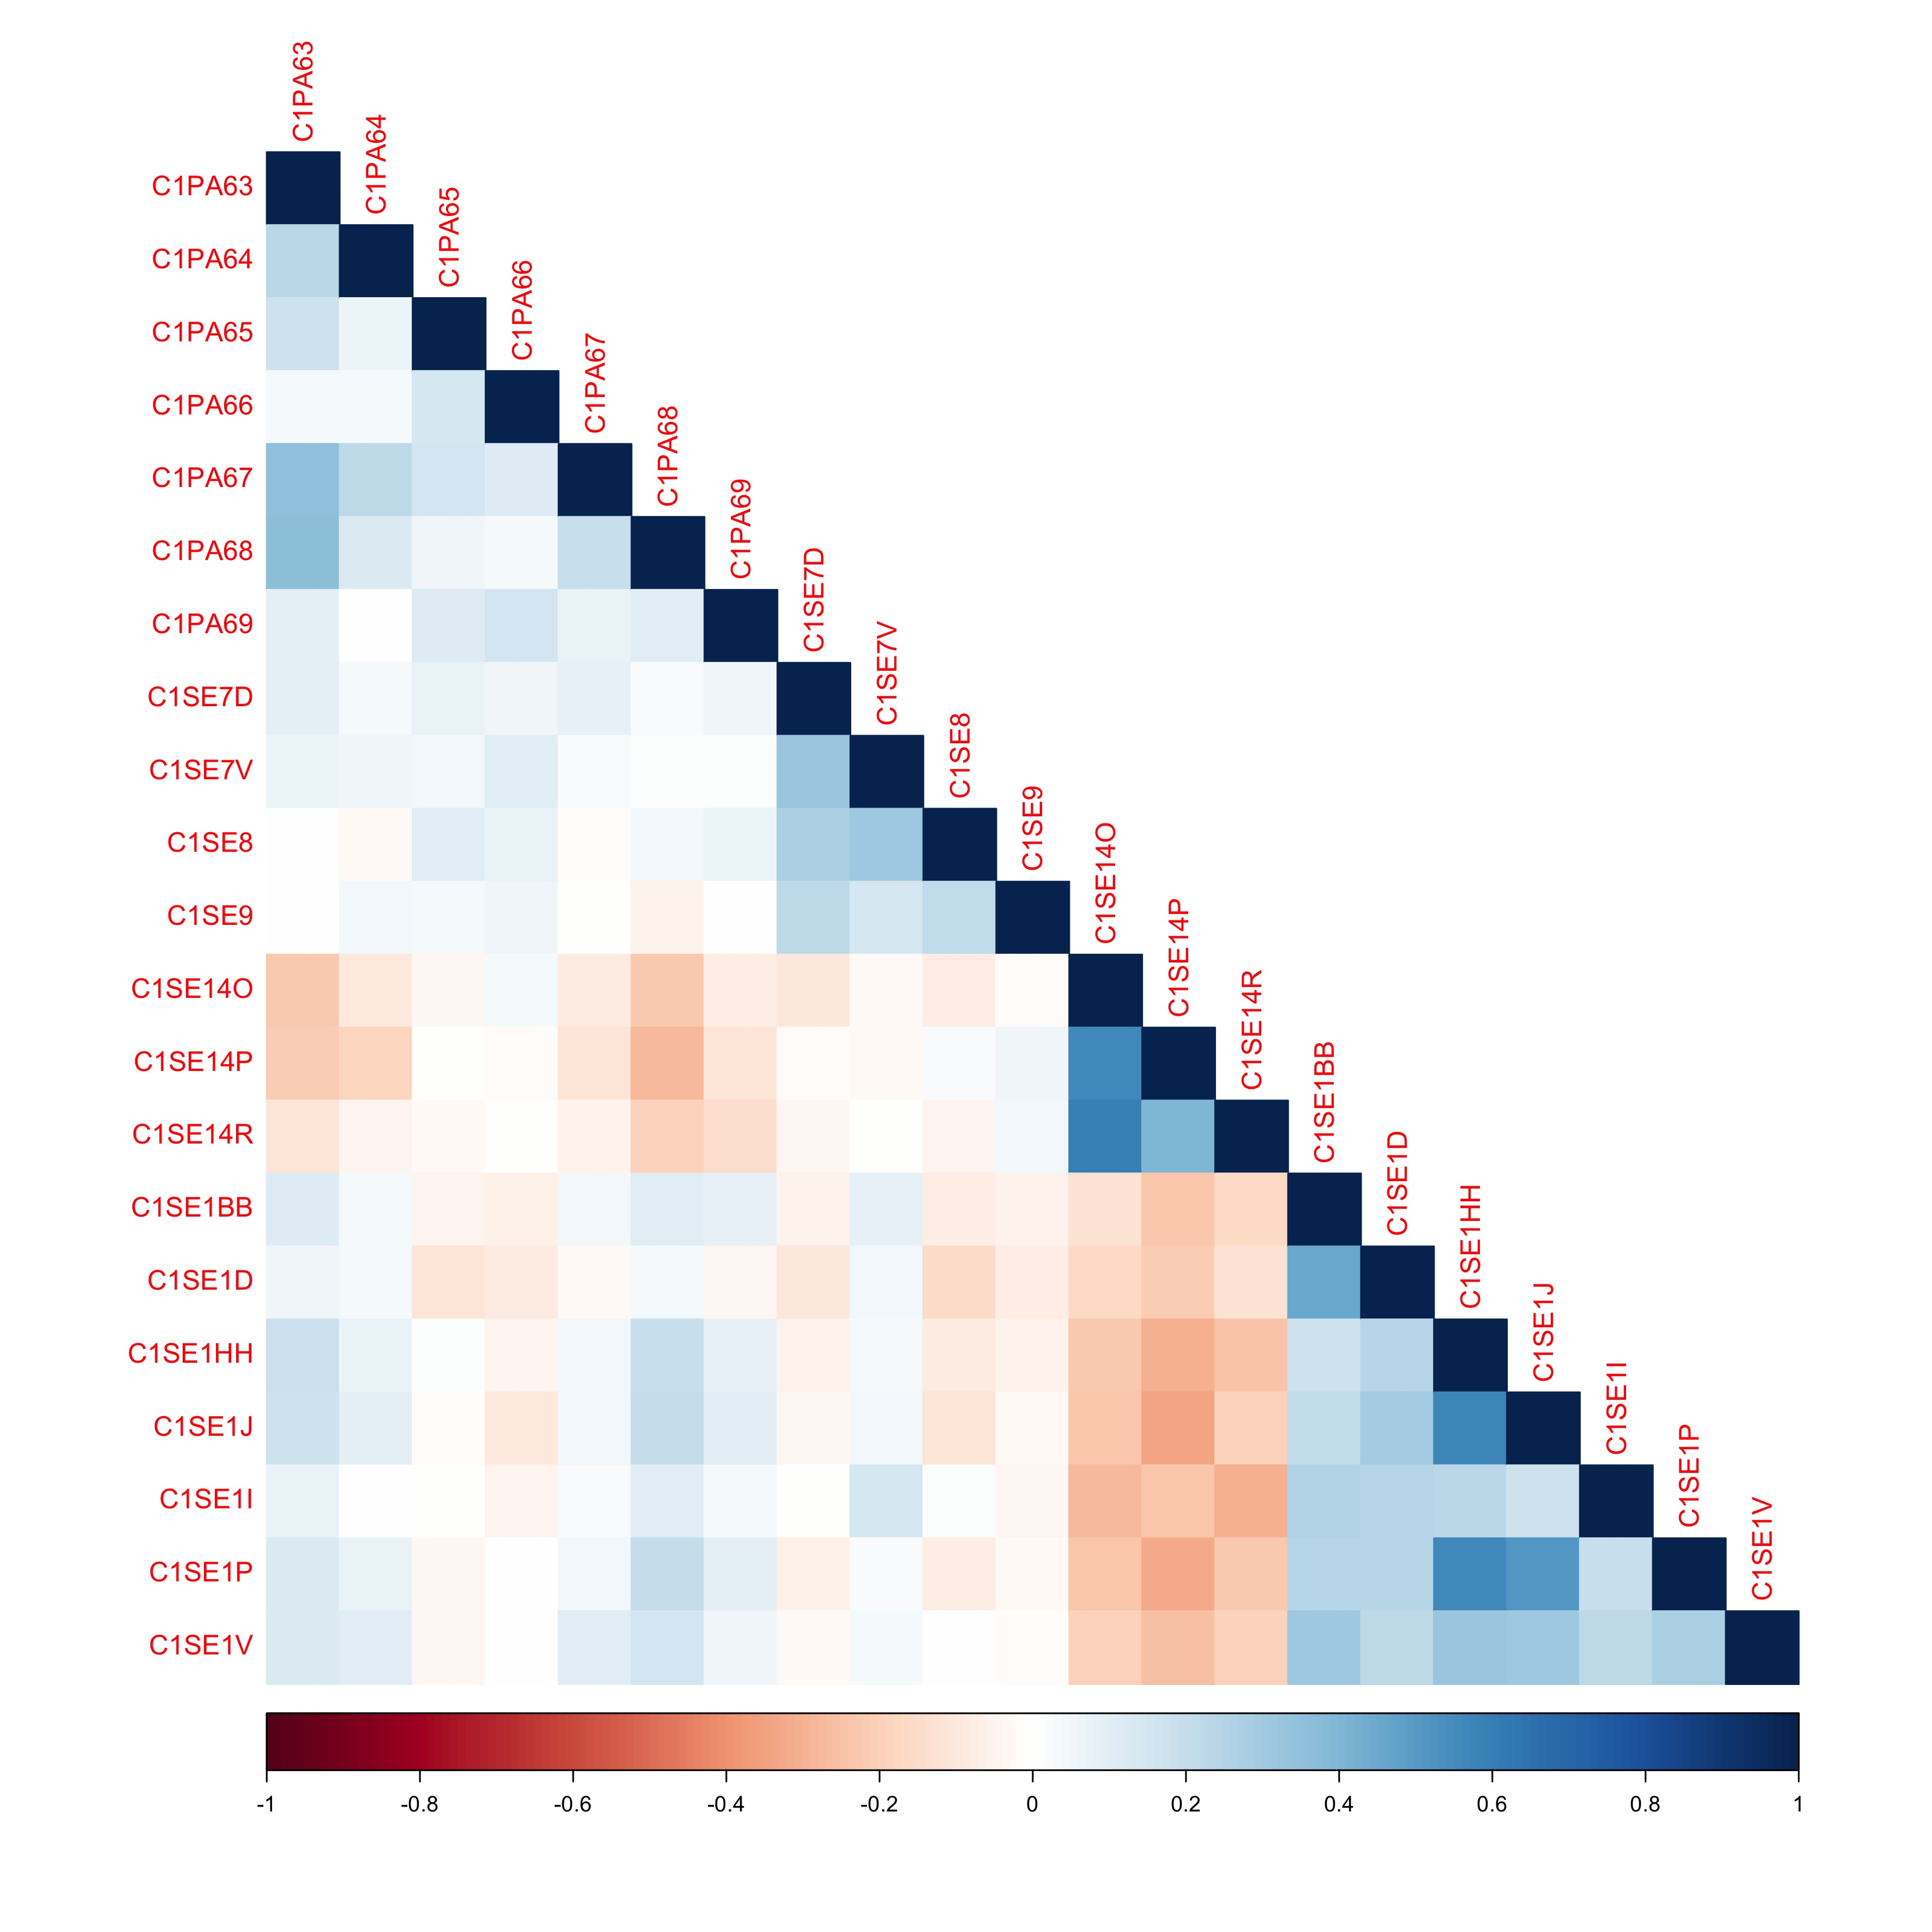
\includegraphics[width=\linewidth]{../visualizations/corr.png}
  \caption{Correlation plot}
  \label{fig:corr}
  \end{minipage}
  \hfill
  \begin{minipage}{0.49\linewidth}
  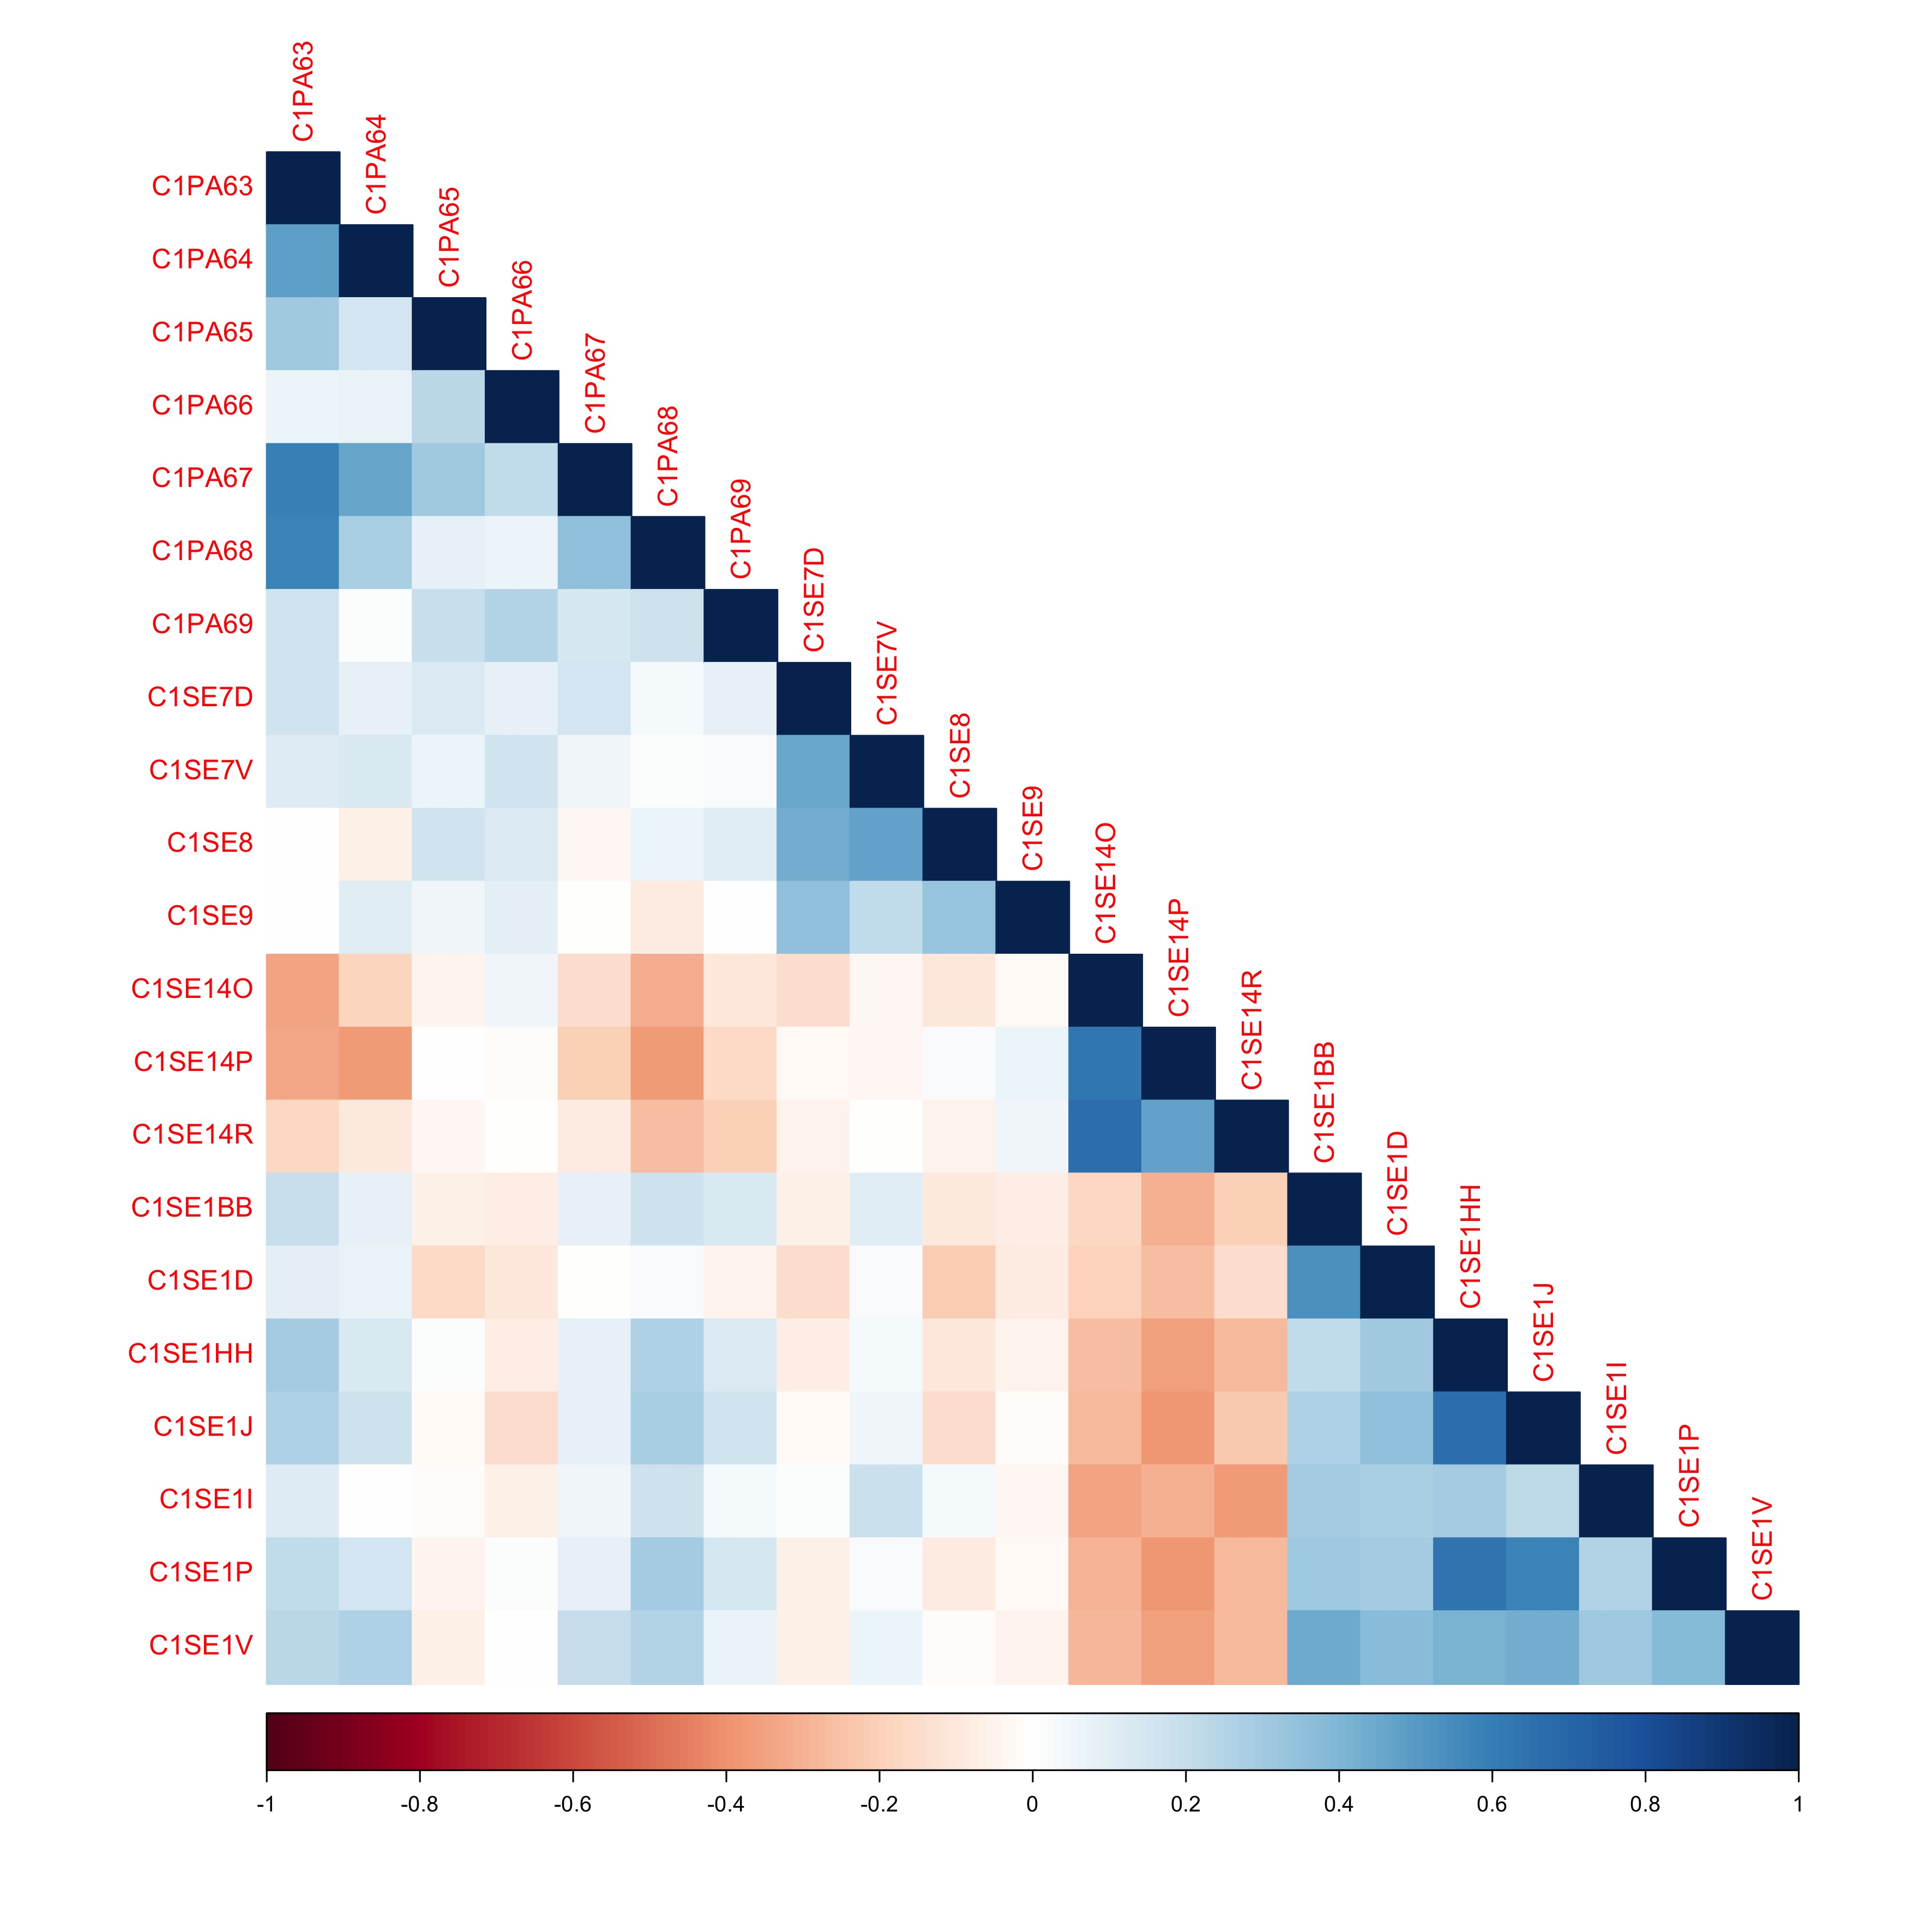
\includegraphics[width=\linewidth]{../visualizations/corr_poly.png}
  \caption{Polychoric correlation plot}
  \label{fig:poly_corr}
  \end{minipage}
\end{figure}

% Missing data

\subsection{Invariance}

% Explain the drop in df

Before continuing any further, it is important to establish the measurement
properties of the model. Test bias, which occurs when items are not measuring
the underlying constructs in the same way across groups, should be avoided at
all costs. By simultaneously putting restrictions on multiple parameters of the
measurement model, such equivalence can be tested (\cite{brown2015}). From the
previous section it is clear that longitudinal data has been used. Are the changes
in a construct then due to changes in the construct itself or due to changes in
how the construct is measured over time? Moreover, other sources of test bias,
specifically the sex and age of the participants, will be tested as well.

Configural invariance is the first step in this process and indicates that the
factor structure is equal across groups. Second, metric invariance is tested by
constraining the factor loadings to be equal across groups. Lastly, by also
constraining the indicator intercepts to be equal, scalar invariance can be
evaluated. A stepwise procedure can be employed by beginning with the least
restricted solution and gradually testing whether the models $\chi^2$ are
significantly different from each other. Essentially, a likelihood ratio test is
used: a rejection of the null hypothesis then indicates that invariance cannot
be concluded and that the more restricted model has a worse fit (\cite{brown2015}).
However, it should be noted that the $\chi^2$ test is sensitive to sample size.
Due to the large sample size in this study, other fit indices will therefore be
used as well. The fit indices will be discussed in more detail later.

\begin{table}[h]
\captionsetup{singlelinecheck=off}
\caption{Gender measurement invariance}
\label{tab:gender_invariance}
\scalebox{0.8}{
\begin{tabular}{|l|l|l|l|l|l|l|l|l|l|}
\hline
\textbf{Invariance form} & $\mathbf{\chi^2}$ & \textbf{df} & $\mathbf{\chi^2}$ \textbf{diff.} & \textbf{df diff.} & \textbf{p-value} & \textbf{RMSEA} & \textbf{SRMR} & \textbf{CFI} & \textbf{TLI} \\ \hline
Configural               & 651.13            & 328         & /                               & /                & /                & 0.057          & 0.090         & 0.956        & 0.949        \\ \hline
Metric                   & 703.46            & 348         & 52.34                           & 20               & \textless{}0.001 & 0.058          & 0.092         & 0.952        & 0.947        \\ \hline
Scalar                   & 727.41            & 384         & 23.95                           & 36               & 0.938            & 0.054          & 0.092         & 0.954        & 0.954        \\ \hline
\end{tabular}
}
\end{table}

First, the invariance of the model with respect to gender will be tested. The
$\chi^2$ difference between the configural and metric model of 52.34 is itself
$\chi^2$ distributed with 20 degrees of freedom. In the metric model there are
20 parameters less to estimate, since there are 20 factor loadings which are
constrained to be equal across the male and female group. Unfortunately, the
p-value associated with the $\chi^2$ test is highly significant (p<0.001), which
indicates that the configural model has a better fit than the metric model. Hence,
metric invariance cannot be concluded based on this test. Next, the $\chi^2$
difference between the metric and scalar model of 23.95 is not significant
(p=0.938). Based on this test, scalar invariance cannot be concluded, since metric
invariance is still a necessary prerequisite. However, other fit measures should
be taken into account due to the large sample size. The RMSEA, CFI and TLI
(equations \ref{eq:rmsea}, \ref{eq:cfi}, \ref{eq:tli}) directly make a correction
for complexity through the degrees of freedom, while the SRMR indirectly makes a
correction through the dimensionality of the reproduced covariance (correlation)
matrix. It is therefore reasonable to expect the fit measures to be more or less
the same for the configural, metric and scalar models if the invariance holds.
Indeed, as shown in Table \ref{tab:gender_invariance} this is the case. I will
therefore conclude that scalar invariance for the male and female group holds.

\begin{table}[h]
\captionsetup{singlelinecheck=off}
\caption{Time measurement invariance}
\label{tab:time_invariance}
\scalebox{0.8}{
\begin{tabular}{|l|l|l|l|l|l|l|l|l|l|}
\hline
\textbf{Invariance form} & $\mathbf{\chi^2}$ & \textbf{df} & $\mathbf{\chi^2}$ \textbf{diff.} & \textbf{df diff.} & \textbf{p-value} & \textbf{RMSEA} & \textbf{SRMR} & \textbf{CFI} & \textbf{TLI} \\ \hline
Configural               & 653.66          & 328         & /                    & /                & /                & 0.057          & 0.092         & 0.956        & 0.949        \\ \hline
Metric                   & 696.43          & 348         & 43.76                & 20               & 0.002            & 0.057          & 0.094         & 0.953        & 0.949        \\ \hline
Scalar                   & 717.76          & 384         & 21.33                & 36               & 0.975            & 0.054          & 0.093         & 0.955        & 0.956        \\ \hline
\end{tabular}
}
\end{table}

Second, the two latest waves of the MIDUS dataset have been combined. The second
wave was collected in 2004 and 2005, while the third wave originates from 2013
and 2014. This source of invariance should be investigated as well, because we
want to be sure that changes in a construct are due to the construct itself and
not because the measurement of the construct has changed over time. Again, we
have to conclude that there is no evidence for metric and scalar invariance based
on the $\chi^2$ test. However, we now know that attention should be paid to other
fit measures due to the large sample size. As shown in Table \ref{tab:time_invariance},
the RMSEA, SRMR, CFI and TLI are very similar for the configural, metric and
scalar models. I will therefore conclude that scalar invariance for the two waves
hold, but it should be noted that the p-value associated with the $\chi^2$ test
is not significant.

\FloatBarrier
\pagebreak
\section{The base model}

Next, the base model will be discussed. Based on the work of \textcite{tse2011},
it has been concluded that depression can be explained through the constructs
harm avoidance, self directedness and social functioning. In other words, there
are four latent variables which are related to each other through a structural
model. Harm avoidance and self-directedness have an effect on social functioning.
Social functioning, then, has an effect on depression. Moreover, it was estimated
that there is also a direct effect of self-directedness on depression.
Hence, there should be no direct effect of harm avoidance on depression.

In the previous section it became clear that ordinal variables have been used in
the analysis. Model identification and estimation will therefore be discussed
first. The measurement model indicates how variables are related to their latent
constructs and will be discussed next. Afterwards, a closer look will be taken
at the structural model, since an important aspect in this work is the
relationships between latent variables. Lastly, the model fit will be evaluated
through fit measures and further inspected using modification indices.

\subsection{Model identification and estimation}

% Model identification
First and foremost, model identification and estimation will be discussed.
A structural equation model is said to be identified if every latent variable
has its scale identified and the models degrees of freedom is zero or greater.
To that end, the scale of the first indicator of every latent variable has been
fixed to one. The model contains 85 parameters that should be estimated.
Specifically, they are 16 ($=20 - 4$) loadings, 4 regression parameters, 60
thresholds (more on this later), 1 latent covariance and 4 latent variances.
The degrees of freedom of the model therefore equals 20*21/2 - 85 = 210 - 85
= 125.
% 20*23/2-85 = 230-85 = 145
% 20*25/2-85 = 250-85 = 165
The following assumptions have been made on the equations shown
in \ref{eq:base_model}. The measurement errors $\delta$ are supposed to have an
expected value of 0. It is assumed that they have constant variance across
observations and are mutually uncorrelated. There should be a covariance of zero
between these errors and the latent variables.

\begin{equation}
    \footnotesize
    \label{eq:base_model}
    \begin{cases}
    \textrm{PA63}  & = \lambda_{11} \textrm{depression} + \delta_{11} \\
    \textrm{PA64}  & = \lambda_{12} \textrm{depression} + \delta_{12} \\
    \textrm{PA65}  & = \lambda_{13} \textrm{depression} + \delta_{13} \\
    \textrm{PA66}  & = \lambda_{14} \textrm{depression} + \delta_{14} \\
    \textrm{PA67}  & = \lambda_{15} \textrm{depression} + \delta_{15} \\
    \textrm{PA68}  & = \lambda_{16} \textrm{depression} + \delta_{16} \\
    \textrm{PA69}  & = \lambda_{17} \textrm{depression} + \delta_{17} \\
    \textrm{SE7V}  & = \lambda_{21} \textrm{harm avoidance} + \delta_{21} \\
    \textrm{SE7D}  & = \lambda_{22} \textrm{harm avoidance} + \delta_{22} \\
    \textrm{SE8}   & = \lambda_{23} \textrm{harm avoidance} + \delta_{23} \\
    \textrm{SE9}   & = \lambda_{24} \textrm{harm avoidance} + \delta_{24} \\
    \textrm{SE14O} & = \lambda_{31} \textrm{self-directedness} + \delta_{31} \\
    \textrm{SE14P} & = \lambda_{32} \textrm{self-directedness} + \delta_{32} \\
    \textrm{SE14R} & = \lambda_{33} \textrm{self-directedness} + \delta_{33} \\
    \textrm{SE1BB} & = \lambda_{41} \textrm{social functioning} + \delta_{41} \\
    \textrm{SE1D}  & = \lambda_{42} \textrm{social functioning} + \delta_{42} \\
    \textrm{SE1HH} & = \lambda_{43} \textrm{social functioning} + \delta_{43} \\
    \textrm{SE1J}  & = \lambda_{44} \textrm{social functioning} + \delta_{44} \\
    \textrm{SE1P}  & = \lambda_{45} \textrm{social functioning} + \delta_{45} \\
    \textrm{SE1V}  & = \lambda_{46} \textrm{social functioning} + \delta_{46} \\
    \textrm{social functioning} & = \beta_1 \textrm{harm avoidance} + \beta_2 \textrm{self-directedness} + \delta_1 \\
    \textrm{depression} & = \beta_3 \textrm{social functioning} + \beta_4 \textrm{self-directedness} + \delta_2
    \end{cases}
\end{equation}

A considerable problem arises when one considers the assumption of multivariate
normality on the residuals $\delta$. All observed variables are ordinal in nature,
meaning that they are not continuous and should not be treated as such. Their
means and (co)variances have no meaning, since they do not have origins or units
of measurement (\cite{joreskog1994}). It would therefore be questionable to
take the usual approach in SEM of modeling the covariance matrix. The standard
maximum likelihood machinery used in SEM is therefore also not applicable. In this
case, robust maximum likelihood or a least squares approach (unweighted least
squares, diagonally weighted least squares or weighted least squares) can be used
(\cite{yangwallentin2010}). The method of diagonally weighted least squares has
been specifically developed for ordinal data and has been shown to yield better
results when the sample size is not small (\cite{li2016}). It has therefore been
applied here. First, polychoric correlations are estimated. Afterwards, the model
parameters can be estimated. 

First, the polychoric correlations should be estimated. A solution can then be
obtained by assuming that a latent, normal variable $x^*$ is responsible for the
observed ordinal variables $x$. With $x=m$ I mean to say that $x$ belongs to a
category $m$. Generally, the mean and variance if $x^*$ are not identified, since
only ordinal information is available (\cite{simsek2012}). They are therefore
fixed to zero and one. Thresholds are used to link the latent variable to its
observed counterpart:

\begin{equation}
  x = m \:\: \text{if} \:\: \nu_m < x^* < \nu_{m+1} .
\end{equation}

Also, if one assumes $x^*$ is standard normally distributed and $\phi$ and $\Phi$
denote the standard normal density and distribution functions:

\begin{equation}
  \pi_m = Pr[x=m] = Pr[\nu_m < x^* < \nu_{m+1}] = \int^{\nu_{m+1}}_{\nu_m} \phi(u)du = \Phi(\nu_{m+1}) - \Phi(\nu_m) .
\end{equation}

In other words, a certain response $m$ from the ordinal variable $x$ is observed,
if the response from its latent variable $x^*$ falls between two thresholds.
Hence, the thresholds are also parameters to be estimated. As far as I am aware,
the polychoric correlations can then be estimated using maximum likelihood.
Afterwards, the model parameters can be estimated using a weighted least squares
approach. The ML and DWLS fit functions are defined as follows:

\begin{align}
  F_{ML} &= \ln |S_{ML}| - \ln |\Sigma| + \text{trace}[(S_{ML})(\Sigma^{-1})] - p \tag{ML fit function} \\
  F_{DWLS} &= [S_{DWLS}-\Sigma]' W^{-1}_D [S_{DWLS}-\Sigma].                      \tag{DWLS fit function}
\end{align}

$S_{ML}$ is the covariance or correlation matrix and $S_{DWLS}$ contains the
polychoric correlations. $\Sigma$ is the reproduced covariance or correlation
matrix and depends on the models parameters. $W_D^{-1}$ is a diagonal weight
matrix, with weights that are inversely proportional to the variances of the
polychoric correlations (\cite{yangwallentin2010}). We can therefore conclude that
both approaches aim at minimizing the difference between a reproduced and sample
covariance or correlation matrix. An important difference, however, is that the
least squares approach allows a weighting for correcting for large polychoric
correlations.

\begin{minipage}{\linewidth}
\begin{lstlisting}
base.model <- "
    # measurement
    depression =~ C1PA63 + C1PA64 + C1PA65 + C1PA66 + C1PA67 + C1PA68 + C1PA69
    harm_avoidance =~ C1SE7V + C1SE7D + C1SE8 + C1SE9
    self_directedness =~ C1SE14O + C1SE14P + C1SE14R
    social_functioning =~ C1SE1BB + C1SE1D + C1SE1HH + C1SE1J + C1SE1P + C1SE1V

    # structural
    social_functioning ~ harm_avoidance+a*self_directedness
    depression ~ b*social_functioning + c*self_directedness
    
    IE := a*b
    TE := c + (a*b) 
"

base.fit <- sem(base.model, data=data, ordered=TRUE, meanstructure=FALSE,
                estimator="DWLS")
summary(base.fit, standardized=TRUE, fit.measures=TRUE)
modindices(base.fit, sort=TRUE, maximum.number=20)
\end{lstlisting}
\end{minipage}

\FloatBarrier
\subsection{Measurement model}

% Measurement model
% More interpretation of loadings here
Second, we will take a closer look at the measurement model, which indicates
how indicators relate to their latent constructs. The factor loading can be
interpreted as the regression slope for predicting the indicator from the latent
variable (\cite{brown2015}). The standardized loading is often more interesting,
since it can be interpreted as a correlation and one does not need to worry
about the scale of the variables. By squaring the standardized loading the
communality can be obtained, which indicates the proportion of the variance in
the indicator that is explained by the latent variable. The residual variance
indicates the proportion of the variance that is not explained by the latent
factor and therefore plays a pivotal role as well. Although there are no hard
rules, a popular cut-off value for the communality appears to be 0.5
(\cite{hair2010}). Hence, more than half of the variance in the indicator should
be explained by the latent variable. Based on my observation, communalities that
are a little bit lower are also acceptable, as long as there is a good
theoretical justification for the relationship between the factor and indicator.
The standardized loading should then be larger than 0.7, which means that the
indicator does a good job at reflecting the latent construct.

%     OK PA63 During those two weeks, did you lose interest in most things?
% NOT OK PA64 Thinking about these same two weeks, did you feel more tired
%             out or low on energy?
% NOT OK PA65 During those same two weeks, did you lose appetite?
% NOT OK PA66 Did you have more trouble falling asleep than you usually do
%             during those two weeks?
% NOT OK PA67 During that same two week period, did you have a lot more
%             trouble concentrating than usual?
%     OK PA68 People sometimes feel down on themselves, no good, or worthless.
%             During that two-week period, did you feel this way?
% NOT OK PA69 Did you think a lot about death - either your own, someone else's
%             or death in general - during those two weeks?

Inspecting Table \ref{tab:measurement_base}, it is evident to see that the
measurement model is lacking in some places.
Using PA63, the respondent was asked about losing interest in most things. The
high standardized loading of 0.850 indicates that the indicator is strongly
correlated with its construct. The same applies to PA68 (participant feels down,
no good or worthless), which has a communality of 0.572. In other words, 57.2\%
of the variance in this indicator is explained by the latent variable.
Unfortunately, we have to conclude that the other depression indicators have a
standardized loading that is too low. Consequently, they are weakly correlated
with their construct and have a residual variance that is too high. 
The variables PA64, PA65, PA66, PA67 and PA69 are the problematic cases. In fact,
the loading associated with PA66 is not even significantly different from zero
(p = 0.136). The indicators PA64, PA65 and PA66 assess feeling low on energy, a
loss of appetite and trouble falling asleep. PA67 and PA69 evaluate trouble
concentrating and often thinking about death. A simple way to improve the model
fit may be to reduce the number of variables that load on depression by deleting
these problematic indicators. However, this action would lead to a decline of
the theoretical support and validity of the model as well (\cite{hair2010}).

\begin{table}[h!]
\captionsetup{singlelinecheck=off}
\caption{Measurement model}
\label{tab:measurement_base}
\scalebox{0.8}{
\begin{tabular}{|l|l|l|l|l|l|l|l|}
\hline
\textbf{Variable} & \textbf{Loading} & \textbf{Standard error} & \textbf{z-value} & \textbf{p-value}     & \textbf{St. loading}           & \textbf{Communality} & \textbf{Unique var.}   \\ \hline
PA63              & 1.000            &                         &                  &                      & 0.850 \hfill ($\lambda_{11}$)  &  0.722               & 0.278 \hfill ($\delta_{11}$)  \\ \hline
PA64              & 0.631            & 0.073                   &  8.662           & \textless 0.001      & 0.536 \hfill ($\lambda_{12}$)  &  0.287               & 0.713 \hfill ($\delta_{12}$)  \\ \hline
PA65              & 0.198            & 0.047                   &  4.236           & \textless 0.001      & 0.168 \hfill ($\lambda_{13}$)  &  0.028               & 0.972 \hfill ($\delta_{13}$)  \\ \hline
PA66              & 0.071            & 0.048                   &  1.492           & 0.136                & 0.061 \hfill ($\lambda_{14}$)  &  0.004               & 0.996 \hfill ($\delta_{14}$)  \\ \hline
PA67              & 0.646            & 0.066                   &  9.757           & \textless 0.001      & 0.548 \hfill ($\lambda_{15}$)  &  0.301               & 0.699 \hfill ($\delta_{15}$)  \\ \hline
PA68              & 0.890            & 0.078                   & 11.460           & \textless 0.001      & 0.757 \hfill ($\lambda_{16}$)  &  0.572               & 0.428 \hfill ($\delta_{16}$)  \\ \hline
PA69              & 0.360            & 0.051                   &  7.005           & \textless 0.001      & 0.306 \hfill ($\lambda_{17}$)  &  0.094               & 0.906 \hfill ($\delta_{17}$)  \\ \hline
%                                                                                                                                
SE7V              & 1.000            &                         &                  &                      & 0.602 \hfill ($\lambda_{21}$)  &  0.362               & 0.637 \hfill ($\delta_{21}$)  \\ \hline
SE7D              & 1.203            & 0.160                   &  7.504           & \textless 0.001      & 0.724 \hfill ($\lambda_{22}$)  &  0.525               & 0.475 \hfill ($\delta_{22}$)  \\ \hline
SE8               & 1.194            & 0.155                   &  7.718           & \textless 0.001      & 0.719 \hfill ($\lambda_{23}$)  &  0.518               & 0.482 \hfill ($\delta_{23}$)  \\ \hline
SE9               & 0.740            & 0.106                   &  7.004           & \textless 0.001      & 0.446 \hfill ($\lambda_{24}$)  &  0.199               & 0.801 \hfill ($\delta_{24}$)  \\ \hline
%                                                                                                                                
SE14O             & 1.000            &                         &                  &                      & 0.821 \hfill ($\lambda_{31}$)  &  0.675               & 0.325 \hfill ($\delta_{31}$)  \\ \hline
SE14P             & 0.982            & 0.049                   & 19.988           & \textless 0.001      & 0.807 \hfill ($\lambda_{32}$)  &  0.651               & 0.349 \hfill ($\delta_{32}$)  \\ \hline
SE14R             & 0.851            & 0.043                   & 19.704           & \textless 0.001      & 0.699 \hfill ($\lambda_{33}$)  &  0.488               & 0.512 \hfill ($\delta_{33}$)  \\ \hline
%                                                                                                                                
SE1BB             & 1.000            &                         &                  &                      & 0.564 \hfill ($\lambda_{41}$)  &  0.318               & 0.682 \hfill ($\delta_{41}$)  \\ \hline
SE1D              & 0.956            & 0.056                   & 17.145           & \textless 0.001      & 0.539 \hfill ($\lambda_{42}$)  &  0.291               & 0.709 \hfill ($\delta_{42}$)  \\ \hline
SE1HH             & 1.398            & 0.066                   & 21.183           & \textless 0.001      & 0.788 \hfill ($\lambda_{43}$)  &  0.621               & 0.379 \hfill ($\delta_{43}$)  \\ \hline
SE1J              & 1.345            & 0.064                   & 21.088           & \textless 0.001      & 0.759 \hfill ($\lambda_{44}$)  &  0.575               & 0.425 \hfill ($\delta_{44}$)  \\ \hline
SE1P              & 1.323            & 0.064                   & 20.568           & \textless 0.001      & 0.746 \hfill ($\lambda_{46}$)  &  0.556               & 0.444 \hfill ($\delta_{46}$)  \\ \hline
SE1V              & 1.113            & 0.060                   & 18.606           & \textless 0.001      & 0.628 \hfill ($\lambda_{47}$)  &  0.394               & 0.606 \hfill ($\delta_{47}$)  \\ \hline
\end{tabular}                                                                                                                                           
}
\end{table}

% SE7D It might be fun and exciting to be in an earthquake.
% SE7V It might be fun learning to walk a tightrope.
% SE8  Of these two situations, I would dislike more: Situation 1:
%      Riding a long stretch of rapids in a canoe; Situation 2:
%      Waiting for someone who's late.
% SE9  Of these two situations, I would dislike more: Situation 1:
%      Being at the circus when two lions suddenly get loose
%      down in the ring; Situation 2: Bringing my whole family
%      to the circus and then not being able to get in because a
%      clerk sold me tickets for the wrong night.
%      => not really a choice between a harm and no harm situation, but between
%         a harm and embarrassment situation

Next, the harm avoidance construct, which measures whether a behaviour is done to
avoid novelty and punishment, plays a central role in this work. It is measured
using four indicators: SE7V, SE7D, SE8 and SE9.
In SE7V the participant is asked whether or not it might be fun to experience an
earthquake. By squaring the standardized loading of 0.602, a low communality of
0.362 is obtained. In other words, there is a moderate correlation between the
indicator and the harm avoidance construct, but the residual variance is too high.
The variable SE7D was formed by asking the interviewee whether or not it might be
fun to learn to walk the tightrope. The standardized loading of 0.724 is high enough.
Next, SE8 and SE9 are used to measure harm avoidance by presenting the respondent
with two situations. Afterwards, a choice has to be made between them. The
standardized loadings are, respectively, 0.729 and 0.446. In the first question
the harmful situation is riding a long stretch of rapids in a canoe, while the
safe situation is waiting for someone who is late. In the second question the
harmful situation is being at the circus when two lions get loose. The safe
situation is bringing the family to the circus, but not being able to get in.
The last question therefore not really presents a choice between a harmful and
a safe situation, but rather a choice between a harmful and an embarrassing
situation. Perhaps this could be the reason why the standardized loading is
lower than in SE9.

% SE14O I like to make plans for the future.
% SE14R I know what I want out of life.
% SE14P I find it helpful to set goals for the near future.

Third, self-directedness has been described as a form of self-determination and
ability to regulate behaviour to suit goals and values. Moreover, it should be
related to the harm avoidance construct (\cite{tse2011}).
The variables SE14O, SE14R and SE14P are used to measure this latent variable.
SE14O evaluates whether or not the respondent likes to make plans for the future.
The standardized loading of 0.821 indicates that there is a high correlation
between the indicator and its latent variable. SE14R is used to measure whether
the participant knows what he or she wants out of life. Again, the standardized
loading of 0.807 is high enough. Lastly, SE14P is used to evaluate whether the
participant finds it helpful to set goals for the near future. The standardized
loading of 0.699 is a bit lower, but still high enough nonetheless.

\begin{figure}[h]
\centering
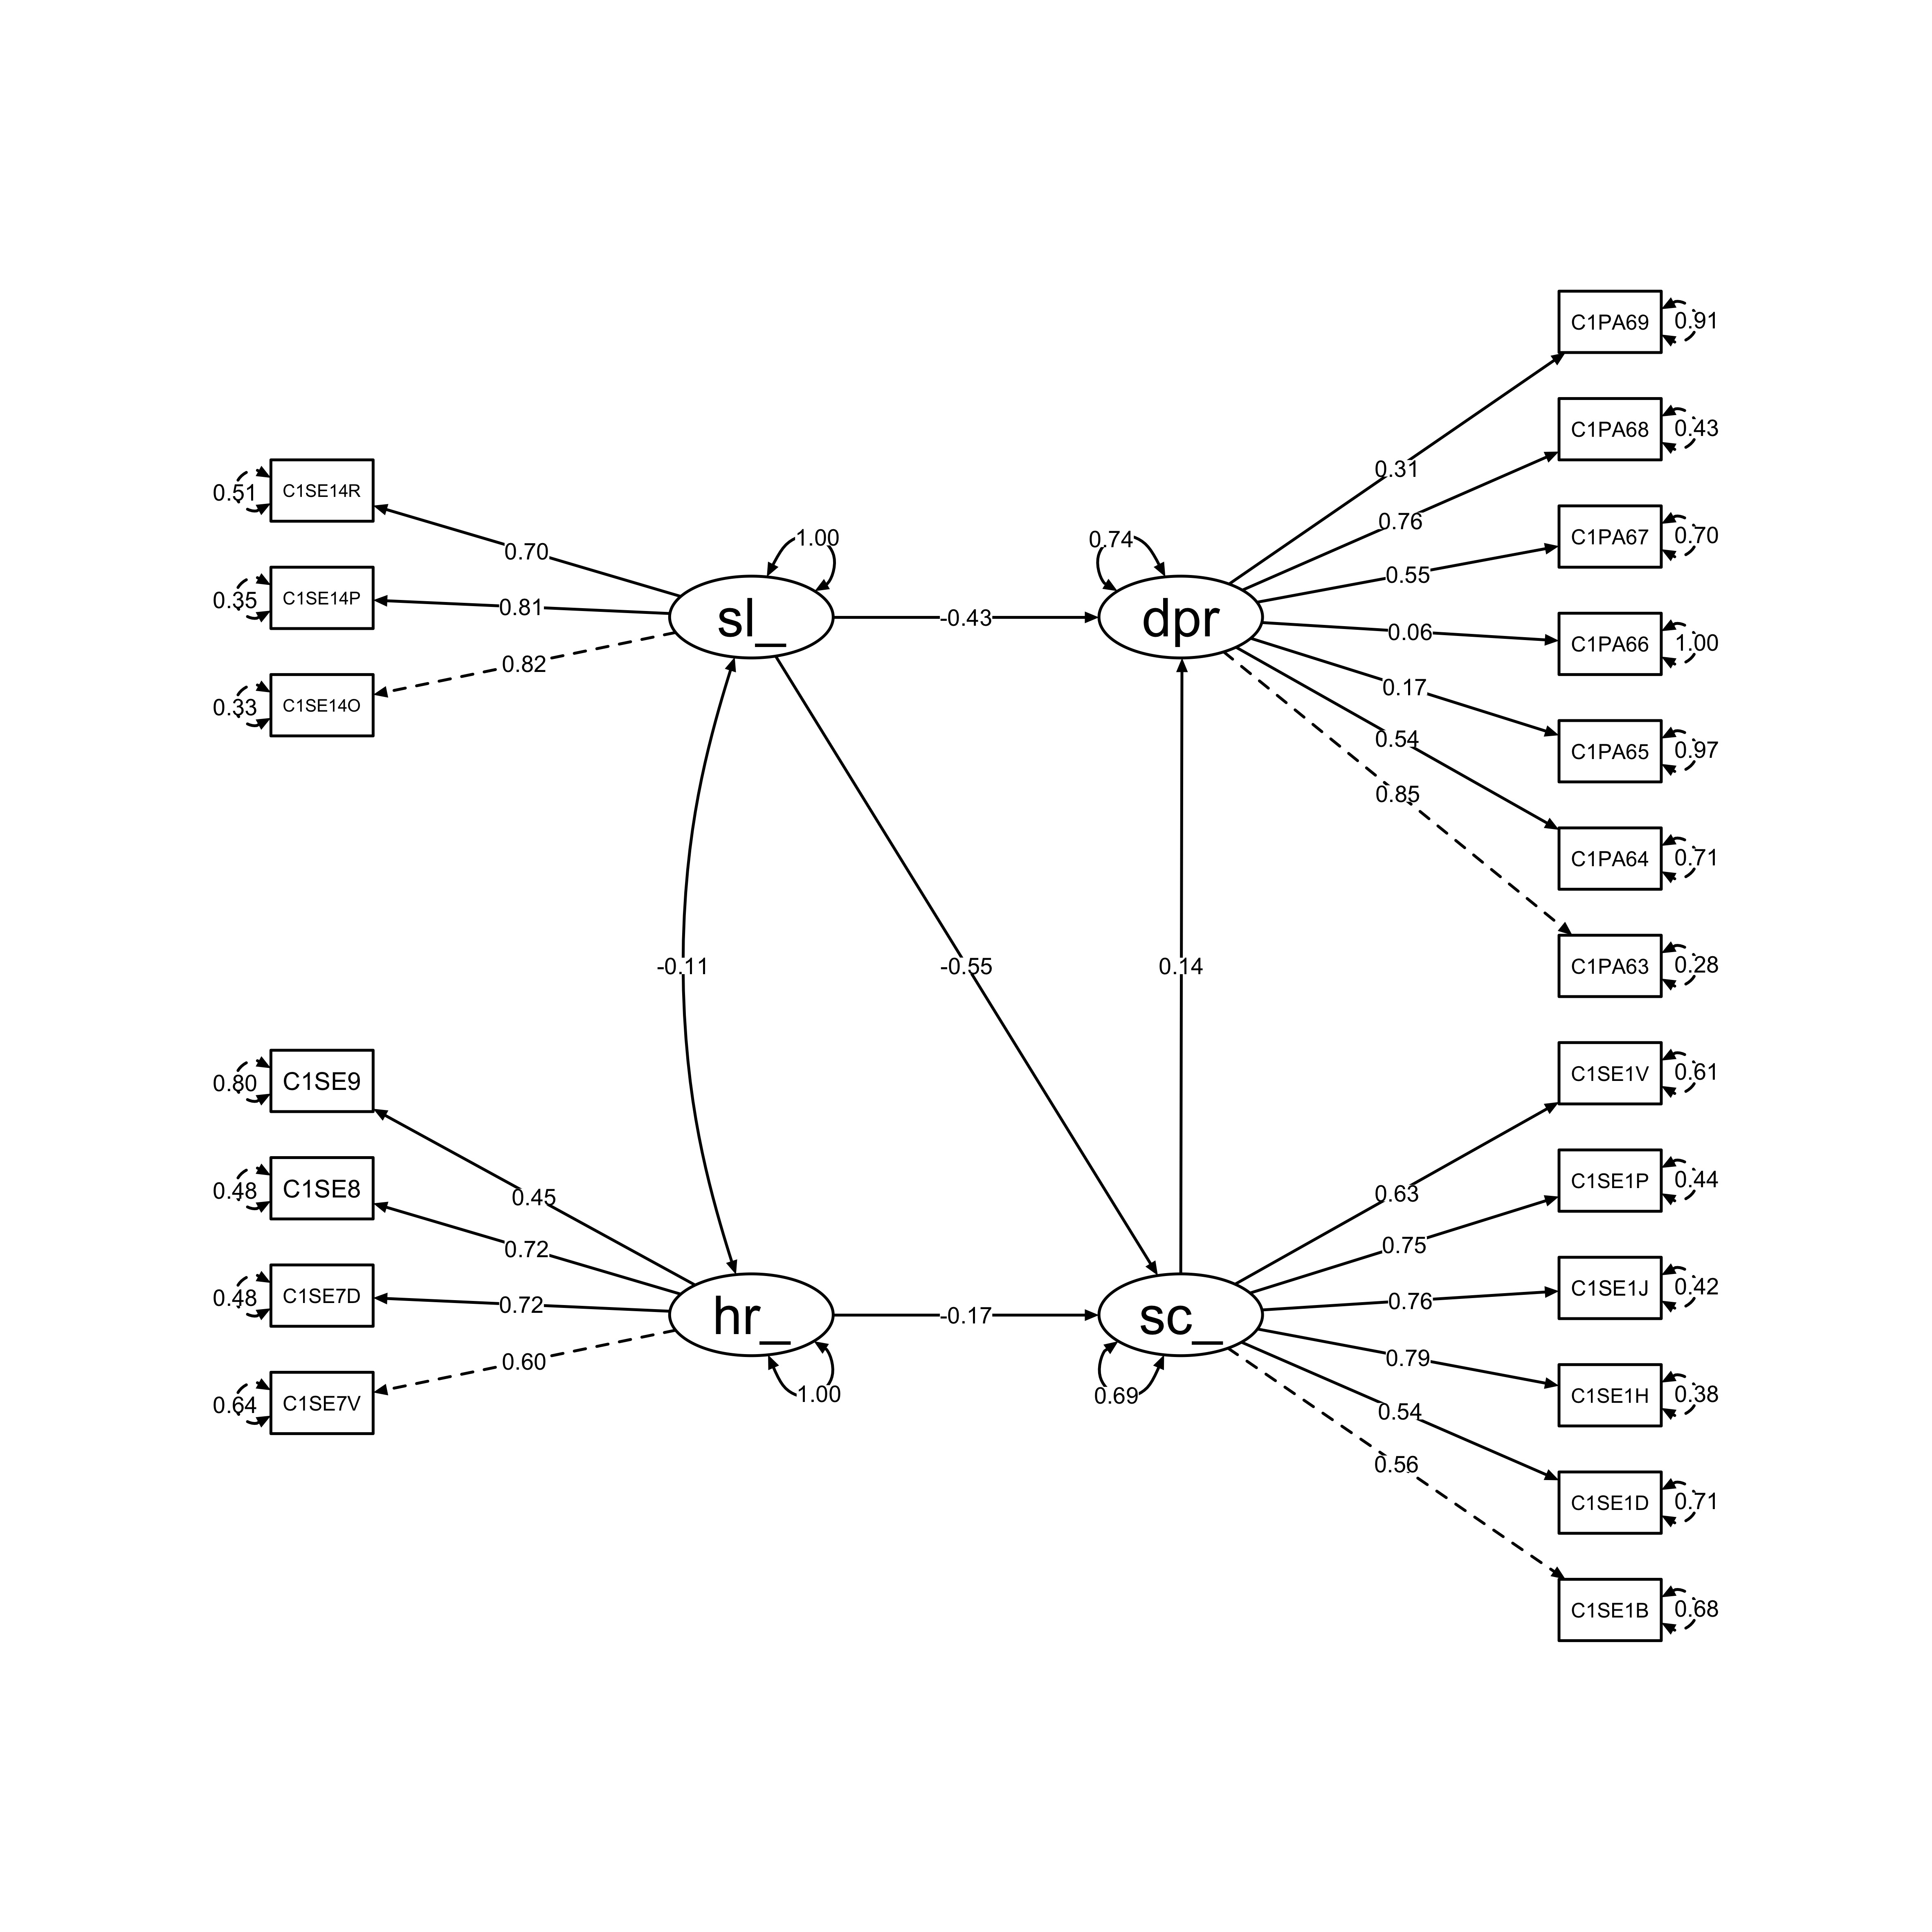
\includegraphics[width=14cm]{../visualizations/base_model.png}
\caption{Summary of the (standardized) base model. hr\_: harm avoidance,
         sl\_: self-directedness, sc\_: social functioning, dpr: depression}
\end{figure}

% SE1BB People would describe me as a giving person, willing to share my time
%       with others.
% SE1D  Most people see me as loving and affectionate.
% SE1HH I have not experienced many warm and trusting relationships with others.
% SE1J  Maintaining close relationships has been difficult and frustrating for me.
% SE1I  I think it is important to have new experiences that challenge how you think
%       about yourself and the world.
% SE1P  I often feel lonely because I have few close friends with whom to share my
%       concerns.
% SE1V  I enjoy personal and mutual conversations with family members and friends.

Lastly, social functioning plays an important role, since it is believed to have
a direct effect on depression (\cite{tse2011}). Seven indicators have been used
to measure this latent variable.
Using SE1BB the respondent was presented with a self-evaluation statement:
`People would describe me as a giving person, willing to share my time with
others.' The standardized loading of 0.564 indicates a poor correlation and a
high residual variance.
The same problem is present in SE1D, which has a standardized loading of 0.539.
SE1HH is used to measure whether the respondent has experienced many warm and
trusting relationships with others. The communality of 0.788 indicates that there
is a high correlation and the indicator does a good job in explaining the variance
of the latent variable.
In SE1J it was asked whether the interviewee has experienced difficulties in
maintaining close relationships. The standardized loading of 0.788 is high enough
and indicates that a one standardized unit increase in social functioning is
estimated to lead to an increase of 0.788 standardized units in SE1J.
Next, SE1P is used to measure whether the respondent often feels lonely because
he or she has few close friends with whom to share his or her concerns. The
standardized loading of 0.746 is high enough.
SE1V is used to evaluate whether the participant enjoys personal and
mutual conversations with family members and friends. The loading is borderline
(0.628), but personally I would still consider it high enough.

To sum up, there are a fair amount of indicators that have a low standardized
loading. Some authors would therefore delete them from the dataset and refit the
model. However, I have decided to leave them in the model, since there is a good
theoretical justification for their relationship with the latent variable.
Furthermore, one needs to take this problem into account when interpreting the
results from the structural model and model evaluation. A chain is only as
strong as its weakest link and in a structural equation model the measurement
model is a very important link.

\FloatBarrier
\subsection{Structural model}

% Structural model
The structural model is of great interest in this work, since it allows us
to make conclusions about the relationships between the latent constructs.
First, we may consider the direct effect of harm avoidance ($\beta_1$) and
self-directedness ($\beta_2$) on social functioning. Both parameters estimates
are highly significant and indicate a negative relationship with social
functioning.
On the one hand, it is estimated that there is a weak, negative relationship
between harm avoidance and social functioning. The standardized regression
coefficient of -0.172 indicates that an increase of one standardized unit in
harm avoidance will lead to a decrease of 0.172 standardized units in social
functioning.
On the other hand, it appears that there is a stronger relationship between
self-directedness and social functioning. This result is a bit counterintuitive,
since the standardized parameter of -0.548 indicates a strong negative
relationship. I would have personally expected a positive relationship between
the two constructs.

Following the theory proposed by \textcite{tse2011}, we may expect there to be
a significant effect of social functioning on depression. Indeed, the results
indicate that there is a negative pattern between the two in the sample, and
this can be generalized to the population (p < 0.001). However, the standardized
coefficient of 0.206 indicates a positive relationship, which is counterintuitive.
In the literature, it is often stated that there is a negative relationship
between the two (\cite{tse2011}).
Lastly, we may consider the direct and indirect effect of self-directedness on
depression. The standardized coefficient of -0.427 indicates a strong negative
direct relationship between the two (p < 0.001). In other words, more
self-directedness is estimated to lead to less depression.
Next, the indirect effect of -0.075 is calculated by multiplying the
standardized parameter estimates of the direct effect of self-directedness on
social functioning ($\beta_2 = -0.548$) and the direct effect of social functioning
on depression ($\beta_3 = 0.136$). 
The total effect (-0.502) can be calculated by adding the direct effect
($\beta_4 = -0.427$) to the indirect effect. The indirect, direct and total
effects are all highly significant (p < 0.001).

\begin{table}[h]
\begin{equation}
\footnotesize
  \begin{cases}
    \textrm{social functioning} & = \beta_1 \textrm{harm avoidance} + \beta_2 \textrm{self-directedness} + \delta_1 \\
    \textrm{depression} & = \beta_3 \textrm{social functioning} + \beta_4 \textrm{self-directedness} + \delta_3
    \tag{Structural model}
  \end{cases}
\end{equation}
\captionsetup{singlelinecheck=off}
\caption{Structural model}
\label{tab:base_structural}
\scalebox{0.8}{
\begin{tabular}{|l|l|l|l|l|l|}
\hline
\textbf{Parameter} & \textbf{Coefficient} & \textbf{Standard error} & \textbf{z-value} & \textbf{p-value} & \textbf{Stand. coefficient} \\ \hline
$\beta_1$          &  -0.161 \hfill       & 0.033                   &  -4.824          & \textless 0.001  & -0.172                      \\ \hline
$\beta_2$          &  -0.376 \hfill       & 0.024                   &  -15.948         & \textless 0.001  & -0.548                      \\ \hline
$\beta_3$          &   0.206 \hfill       & 0.064                   &   3.214          & 0.001            &  0.136                      \\ \hline
$\beta_4$          &  -0.442 \hfill       & 0.056                   &  -7.956          & \textless 0.001  & -0.427                      \\ \hline
\end{tabular}
}
\end{table}

Moreover, the latent variables social functioning and depression have a residual
variance, since they are not exogenous in nature. In the standardized solution,
the residual variance indicates the portion of the variance that is not accounted
for by the latent variable. Both depression and social functioning have a high
residual variance: 0.737 and 0.690, respectively. This insight indicates that
something is not entirely correct with the model, since these residual covariances
should be lower if the latent variables are being predicted correctly.

Strongly related to the structural model is the notion of discriminant validity.
Discriminant validity gives an indication that theoretically different constructs
should not be highly intercorrelated. In other words, if two latent variables
are highly correlated they could represent the same construct and they could be
merged into one latent variable to obtain a more parsimonious solution
(\cite{brown2015}). The low and insignificant (p=0.108) standardized covariance
or correlation of -0.1 between harm avoidance and self-directedness indicates
that there is little evidence for poor discriminant validity.

\pagebreak
\subsection{Goodness of fit}

Fourth, the goodness of fit of the model will be evaluated using $\chi^2$, SRMR,
RMSEA, CFI and TLI. The sources of misfit will be further investigated using
modification indices. It was previously concluded that there are some problems
with the measurement model. The structural model seemed fine, but the results
were a bit counterintuitive. This evaluation step is therefore crucial to
further determine if the model is a good fit for the data or not.

\subsubsection{Test statistics}

% Goodness of fit
The $\chi^2$ statistic is closely related to the fit of the model and is very
popular in the literature, but it has received some important criticisms.
It has been noted that it is inflated by sample size and in many instances the
underlying distribution is not $\chi^2$ distributed (\cite{brown2015}).
In this illustration, the test statistic of 505.23 is larger than the critical
value of 105.52. Hence, the null hypothesis that this model is equal to a
perfectly fitting model can be rejected and poor model fit is concluded. However,
given the large sample size this result should not be trusted.

% Absolute fit
Absolute fit indices have therefore been employed. They assess the quality of
the solution without taking into account model parsimony. First, the standardized
root mean square residual (SRMR) can be interpreted as the square root average
standardized residual covariance (polychoric correlation). It can be calculated
using the following equation, where $p$ is the number of indicators and $\epsilon$
is the vector of the standardized residual covariances (\cite{shi2020}). In this
illustration a SRMR of 0.081 was obtained, which indicates borderline poor model
fit as it is just above the target of 0.08.

\begin{minipage}{0.48\linewidth}
\begin{equation}
\label{eq:srmr}
  SRMR = \sqrt{\dfrac{\epsilon \epsilon}{p(p+1)/2}}
\end{equation}
\end{minipage}
\begin{minipage}{0.48\linewidth}
\begin{equation}
\label{eq:rmsea}
  RMSEA = \sqrt{\dfrac{\chi^2 - df}{N \times df}}
\end{equation}
\end{minipage}

Second, the root mean square error of approximation (RMSEA) is based on the
$\chi^2$ statistic and takes into account the error of approximation in the
population. The RMSEA takes values between zero and one and the fit of the model
is acceptable if it falls under 0.05. A borderline unacceptable fit is obtained
with a RMSEA of 0.058.

% Comparative fit
The CFI and TLI are two comparative fit indices that will be evaluated as well.
This group of statistics is called comparative, since they make a comparison
between a restricted null model and an alternative model supplied by
the model-builder (\cite{brown2015}). The comparative fit index (CFI) and
Tucker-Lewis index (TLI) have been shown below. Both measures have a range of
possible values from zero to one and make a correction for complexity through
the degrees of freedom. Values that are close to one imply a good model fit,
since the alternative and null model will then be close to each other.
Generally, 0.9 is taken as a target value. In this work the CFI and TLI
are, respectively, 0.952 and 0.945. To sum up, the fit of this model is
borderline good or bad, depending on which fit measures are taken into account.

\begin{minipage}{0.48\linewidth}
\begin{equation}
\label{eq:cfi}
    CFI = \dfrac{(\chi^2 - df)_{null} - (\chi^2 - df)_{alternative}}{(\chi^2 - df)_{null}}
\end{equation}
\end{minipage}
\begin{minipage}{0.48\linewidth}
\begin{equation}
\label{eq:tli}
    TLI = \dfrac{(\chi^2 / df)_{null} - (\chi^2 / df)_{alternative}}{(\chi^2 / df)_{null}}
\end{equation}
\end{minipage}

\begin{table}[h!]
\captionsetup{singlelinecheck=off}
\caption{Test statistics}
\scalebox{0.8}{
\begin{tabular}{|l|l|l|}
\hline
\textbf{Statistic} & \textbf{Value} & \textbf{Target}   \\ \hline
$\chi^2$           & 505.23         & < 105.52          \\ \hline
CFI                & 0.952          & > 0.9             \\ \hline
TLI                & 0.945          & > 0.9             \\ \hline
RMSEA              & 0.058          & < 0.05            \\ \hline
SRMR               & 0.081          & < 0.08            \\ \hline
\end{tabular}
}
\end{table}

\begin{table}[h!]
\captionsetup{singlelinecheck=off}
\caption{The 10 highest modification indices of base model}
\label{tab:base_modification}
\scalebox{0.8}{
\begin{tabular}{|l|l|l|l|l|l|}
\hline
\textbf{Left hand side} & \textbf{Operation} & \textbf{Right hand side} & \textbf{Modification index} & \textbf{\begin{tabular}[c]{@{}l@{}}Expected parameter\\ change\end{tabular}} & \textbf{\begin{tabular}[c]{@{}l@{}}Stand. expected\\ parameter change\end{tabular}} \\ \hline
C1SE1BB                 & correlation        & C1SE1D                   & 90.619                      &  0.329                                                                       &  0.473 \\ \hline
C1SE14O                 & correlation        & C1SE14R                  & 44.130                      &  0.317                                                                       &  0.778 \\ \hline
social\_functioning     & loading            & C1SE14P                  & 36.950                      & -0.551                                                                       & -0.311 \\ \hline
C1SE1BB                 & correlation        & C1SE1HH                  & 34.474                      & -0.290                                                                       & -0.570 \\ \hline
social\_functioning     & loading            & C1PA65                   & 29.688                      & -0.415                                                                       & -0.234 \\ \hline
social\_functioning     & loading            & C1PA66                   & 26.101                      & -0.403                                                                       & -0.227 \\ \hline
social\_functioning     & loading            & C1SE14O                  & 22.440                      &  0.463                                                                       &  0.261 \\ \hline
depression              & loading            & C1SE1D                   & 20.018                      & -0.253                                                                       & -0.215 \\ \hline
social\_functioning     & loading            & C1SE7V                   & 19.761                      &  0.255                                                                       &  0.144 \\ \hline
C1SE1HH                 & correlation        & C1SE1J                   & 19.647                      &  0.170                                                                       &  0.424 \\ \hline
\end{tabular}                                                                                                    
}
\end{table}

\subsubsection{Modification indices}

The modification indices can be used to more precisely investigate sources of
model misfit. They can be calculated for each fixed and constrained parameter in
the model and indicate how much the model $\chi^2$ would drop if a certain
parameter were to be freely estimated. A good fitting model should then also
produce modification indices that are small in magnitude. A modification index
that is greater than 3.84 indicates that the model fit can be significantly
improved if the parameter is freely estimated (\cite{brown2015}). Unfortunately,
the summary shown in Table \ref{tab:base_modification} indicates that there are
various sources of badness of fit associated with the measurement model. The
question is now how to proceed. Since structural equation modeling is at heart
a theory testing framework, it is important to first investigate the reason why
a certain modification index is too large. A proper theoretical justification
needs to be present before freeing a parameter.

% 1SE1BB <=> SE1D: YES
First, a huge drop in the model's $\chi^2$ of 90.62 can be realized by allowing
a correlated error term between the variables 1SE1BB and SE1D, which share a
loading on social functioning. On the one hand, SE1BB assesses whether the 
respondent believes other people would describe him/her as a giving person.
On the other hand, SE1D evaluates whether the respondent believes other people
see him/her as loving and affectionate. Personally, I believe that it is very
plausible that these two variables are related to one another. A correlation
between these variables will therefore be allowed in the improved model.

% 1SE14O <=> 1SE14R: NO
Next, the modification indices indicate that the model fit would improve
dramatically should a correlated error term be allowed between the
self-directedness variables 1SE14O and 1SE14R. In 1SE14O and 1SE14R it is asked
whether the respondent likes to make plans for the future and knows what to want
out of life, respectively. Personally, I cannot see how these variables would be
directly related to each other.

% social functioning =~ 1SE14P
Third, it is suggested that cross-loading can be allowed in the model to improve
its fit. Specifically, the variable SE14P is suggested to load on social
functioning. In 1SE14P it is asked whether the interviewee likes to make plans
for the future. Clearly, this variable is more related to self-directedness than
social functioning. Allowing such a cross-loading would also make the structural
model more difficult to interpret.

% 1SE1HH <=> 1SE1BB
Additionally, the modification indices indicate that a correlated error term
should be allowed between the variables 1SE1HH and 1SE1BB. Both variables have a
loading on social functioning. 1SE1HH indicates whether the respondent has
experienced many warm and trusting relationships. 1SE1BB assesses whether the
respondent believes he or she would be described by others as a giving person,
willing to share his or her time. Personally, I cannot see how both variables are
directly related to each other.

\FloatBarrier
\pagebreak
\section{Expanding the base model}

\FloatBarrier
\pagebreak
\section{Conclusion}

\end{document}
